\documentclass{beamerperso}
% \usetikzlibrary{external}
% \tikzexternalize[prefix=tikz/]
\usepackage{tikz}
\usepackage{bookmark}
\usetikzlibrary{plotmarks}
\usepackage{graphicx}
\usepackage{pdfrender}
\usepackage{pifont}
\newcommand*{\MarkSymbol}[3]{%
  \textpdfrender{%
    TextRenderingMode=FillStroke,
    LineWidth=.4pt,
    FillColor={#2},
    StrokeColor={#3},
  }{\scriptsize\ding{#1}}%
}
\newcommand*{\BlueRoute}{%
  \rotatebox{45}{%
    \MarkSymbol{110}{blue!60!white}{blue!80!black}%
  }%
}
\newcommand*{\WhiteSquare}{%
  \MarkSymbol{110}{white}{gray}%
}
\newcommand*{\RedStar}{%
  \MarkSymbol{72}{red!60!white}{red!80!black}%
}
\newcommand*{\GreenStar}{%
  \MarkSymbol{72}{green!60!white}{green!80!black}%
}
\newcommand*{\GreenCirc}{%
  \MarkSymbol{108}{green!80!white}{green!80!black}%
}
\newcommand*{\BlackCirc}{%
  \MarkSymbol{108}{black}{black}%
}

\newcommand*{\baseGraph}{
  % Lines
  \draw[black]
    \foreach \x in {-5,..., 4} {
      (\x, -3) -- (\x,6) 
    }
    \foreach \x in {-3, ..., 4} { % gauche à droite
     (\x, -3) -- (\x,8) 
    }
    
    \foreach \y in {7,8} {
      (-3, \y) -- (4, \y)
    }
    \foreach \y in {-3, ..., 6} { % du bas vers le haut
      (-5, \y) -- (4, \y)
    }
    %%%%%__________ 1 in matrix __________
    \foreach \x in {-2.5,-1.5,...,3.5}{
        (\x, 5.5) node{$1$}
        (\x, 4.5) node{$1$}
    }
    \foreach \x in {-1.5,-0.5,...,3.5}{
        (\x, 3.5) node{$1$}
        (\x, 2.5) node{$1$}
        (\x, 1.5) node{$1$}
    }
    \foreach \x in {0.5,1.5,...,3.5}{
        (\x, 0.5) node{$1$}
    }
    \foreach \x in {1.5,2.5,...,3.5}{
        (\x, -0.5) node{$1$}
    }
    %%%%%__________ 0 in matrix __________
     \foreach \x in {-2.5,-1.5,...,3.5}{
        (\x, -1.5) node{$0$}
        (\x, -2.5) node{$0$}
    }
    \foreach \x in {-2.5,-1.5,...,0.5}{
        (\x, -0.5) node{$0$}
    }
    \foreach \x in {-2.5,-1.5,...,-0.5}{
        (\x, 0.5) node{$0$}
    }
    \foreach \x in {0.5,1.5,...,3.5}{
        (-2.5, \x) node{$0$}
    }
  ;
  %%%%%___________ deliminting lines 
  \draw[line width=1, red,->](-5,6) -- (4.5,6);
  \draw[line width=1, red,->](-3,8) -- (-3,-3.5);
    \node[anchor=south] at (4.5,6.1) {\Huge{\color{red}x}};
    \node[anchor=east] at (-3,-3.35) {\Huge{\color{red}y}};
  %%%%%%%%__________________________
  
  %%%%%%%%%___________________ Diagonal lines
  \draw[line width=0.5, black!30, dotted]
  \foreach \i in {0,...,9}{
  (-3,-3+\i)--(6-\i,6)}
  \foreach \i in {0,...,9}{
  (-3+\i,-3)--(6,6-\i)}
;
  % Annotations
  
  \node at (-4.5,5.5) {$A[0]$};
  \node at (-4.5,4.5) {$A[1]$};
  \node at (-4.5,3.5) {$A[2]$};
  \node at (-4.5,2.5) {$A[3]$};
  \node at (-4.5,1.5) {$A[4]$};
  \node at (-4.5,0.5) {$A[5]$};
  \node at (-4.5,-0.5) {$A[6]$};
  \node at (-4.5,-1.5) {$A[7]$};
  \node at (-4.5,-2.5) {$A[8]$};
  
  \node at (-3.5,5.5) {1};
  \node at (-3.5,4.5) {2};
  \node at (-3.5,3.5) {5};
  \node at (-3.5,2.5) {6};
  \node at (-3.5,1.5) {6};
  \node at (-3.5,0.5) {9};
  \node at (-3.5,-0.5) {11};
  \node at (-3.5,-1.5) {15};
  \node at (-3.5,-2.5) {16};
  
  
  
 
  
  \node at (-2.5,7.5) {$B[0]$};
  \node at (-1.5,7.5) {$B[1]$};
  \node at (-0.5,7.5) {$B[2]$};
  \node at (0.5,7.5) {$B[3]$};
  \node at (1.5,7.5) {$B[4]$};
  \node at (2.5,7.5) {$B[5]$};
  \node at (3.5,7.5) {$B[6]$};

  \node at (-2.5,6.5) {4};
  \node at (-1.5,6.5) {7};
  \node at (-0.5,6.5) {8};
  \node at (0.5,6.5) {10};
  \node at (1.5,6.5) {12};
  \node at (2.5,6.5) {13};
  \node at (3.5,6.5) {14};
  
 
}

\newcommand*{\maze}{
\path [draw,line width=0.2cm,color=blue!30,cap=round,join=round]
}
% --------------------------------------------------- %
%                  Presentation info	              %
% --------------------------------------------------- %
\title[HPCA]{Project GPU : Path merge}
\subtitle{}
\author[MAIN5--Path merge]{
Arthur \textbf{Zucker} ,
Clément  \textbf{Apavou}}
\institute[Polytech Sorbonne]{
\begin{figure}[!h]
    \minipage{0.5\textwidth}
    \centering
     
\includegraphics[width=0.7\linewidth]{image/polytech_sorbonne.jpg}
    \endminipage
    \minipage{0.5\textwidth}
    \centering
     
\includegraphics[width=0.7\linewidth]{image/SU_SCIENCES-removebg-preview.png}
    \endminipage
\end{figure}
}

\subject{ClusTi} % metadata
\begin{document}

%%%%%%%%%%%%%%%%%%%%%%%%%%%%%%%%%%%%%%%%%%%%%%%%%
\begin{frame}
\titlepage
\end{frame}
%%%%%%%%%%%%%%%%%%%%%%%%%%%%%%%%%%%%%%%%%%%%%%%%%

%%%%%%%%%%%%%%% Table of contents %%%%%%%%%%%%%%% 
\begin{frame}{Table des matières}
\setcounter{tocdepth}{1}
\tableofcontents    
\end{frame}
%%%%%%%%%%%%%%%%%%%%%%%%%%%%%%%%%%%%%%%%%%%%%%%%%

%%%%%%%%%%%%%%%%%%%%%%%%%%%%%%%%%%%%%%%%%%%%%%%%%
\section{Introduction}
\begin{frame}{Introduction}
\begin{block}{Keywords}
    CUDA · Stream · Merging
\end{block}
\begin{itemize}
    \item We have to finish the code
    \item  Then work on the report
    \item Finally work on the beamer 
\end{itemize}
\end{frame}
%%%%%%%%%%%%%%%%%%%%%%%%%%%%%%%%%%%%%%%%%%%%%%%%%

\begin{frame}{Path merged : thread 0}
    \setbeamercovered{invisible}
\RaggedRight
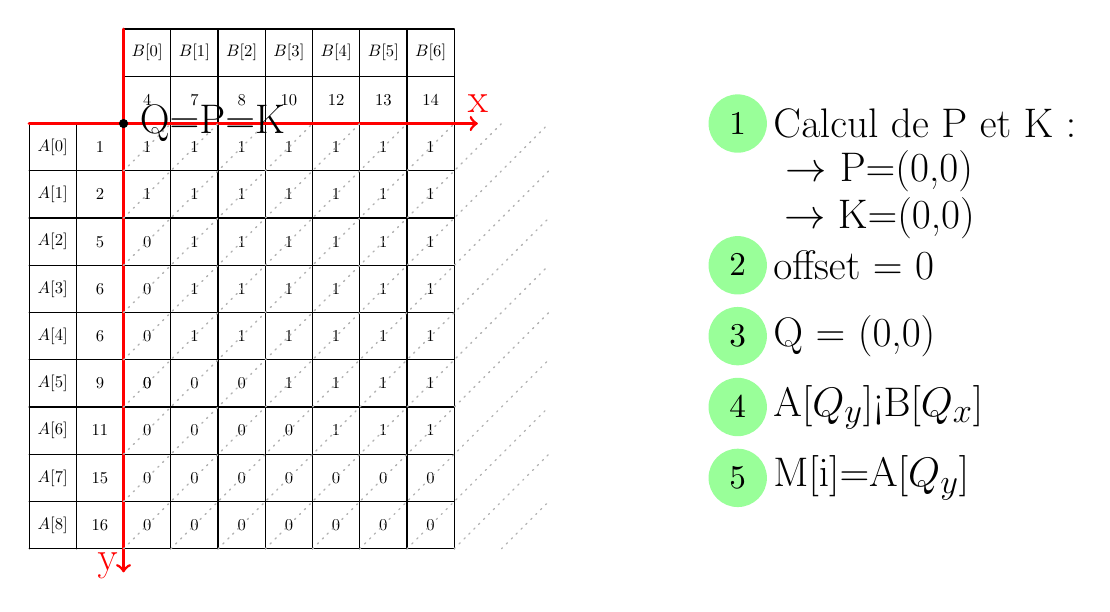
\begin{tikzpicture}[line cap=round,scale=0.6, every node/.style={transform shape}]
    \baseGraph
    \draw (10,6) node[shape = circle,label=right:\Huge{Calcul de P et K :},fill=green!40,scale=2] {1}; \pause
    \draw (13,5) node {\Huge{$\rightarrow$ P=(0,0)}};\pause
    \draw (13,4) node {\Huge{$\rightarrow$ K=(0,0)}};\pause
    \draw (10,3) node[shape = circle,label=right:\Huge{offset = 0},fill=green!40,scale=2] {2}; \pause
    \draw (10,1.5) node[shape = circle,label=right:\Huge{Q = (0,0)},fill=green!40,scale=2] {3}; 
    \draw  (-3,6) node[label=right:\Huge{Q=P=K}] {\BlackCirc};\pause
    \draw (10,0) node[shape = circle,label=right:\Huge{A[$Q_{y}$]<B[$Q_{x}$]},fill=green!40,scale=2] {4};\pause 
    \draw (10,-1.5) node[shape = circle,label=right:\Huge{M[i]=A[$Q_{y}$]},fill=green!40,scale=2] {5}; 
    %\draw (-3,6) node {\BlueRoute}; \pause
\end{tikzpicture}
\end{frame}

\begin{frame}{Path merged : thread 0,path}
    \setbeamercovered{invisible}
\RaggedRight
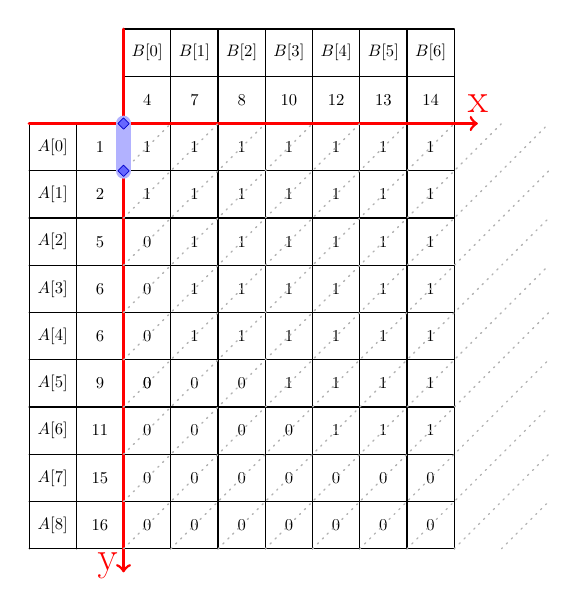
\begin{tikzpicture}[line cap=round,scale=0.6, every node/.style={transform shape}]
    \baseGraph
    \draw (-3,6) node {\BlueRoute}; \pause
    \maze (-3,6) node {\BlueRoute}--(-3,5)node {\BlueRoute};
\end{tikzpicture}
\end{frame}
\begin{frame}{Path merged : thread 1}
    \setbeamercovered{invisible}
\RaggedRight
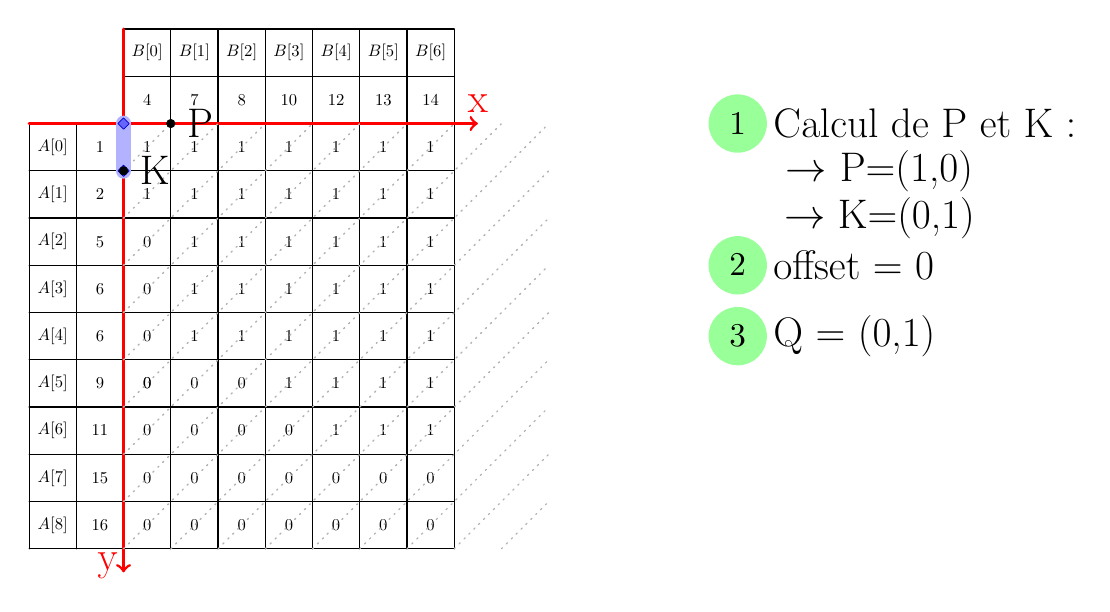
\begin{tikzpicture}[line cap=round,scale=0.6, every node/.style={transform shape}]
    \baseGraph
    \maze (-3,6) node {\BlueRoute}--(-3,5)node {\BlueRoute}; %ajouter ce qu'on a déjà fait 
    \draw (10,6) node[shape = circle,label=right:\Huge{Calcul de P et K :},fill=green!40,scale=2] {1}; \pause
    \draw (13,5) node {\Huge{$\rightarrow$ P=(1,0)}}; 
    \draw (-2,6) node[label=right:\Huge{P}] {\BlackCirc};\pause

    \draw (13,4) node {\Huge{$\rightarrow$ K=(0,1)}};
    \draw (-3,5) node[label=right:\Huge{K}] {\BlackCirc};\pause
    \draw (10,3) node[shape = circle,label=right:\Huge{offset = 0},fill=green!40,scale=2] {2};\pause
    \draw (10,1.5) node[shape = circle,label=right:\Huge{Q = (0,1)},fill=green!40,scale=2] {3}; 
    %\draw (-3,6) node {\BlueRoute}; \pause
\end{tikzpicture}
\end{frame}

\begin{frame}{Path merged : thread 1}
    \setbeamercovered{invisible}
\RaggedRight
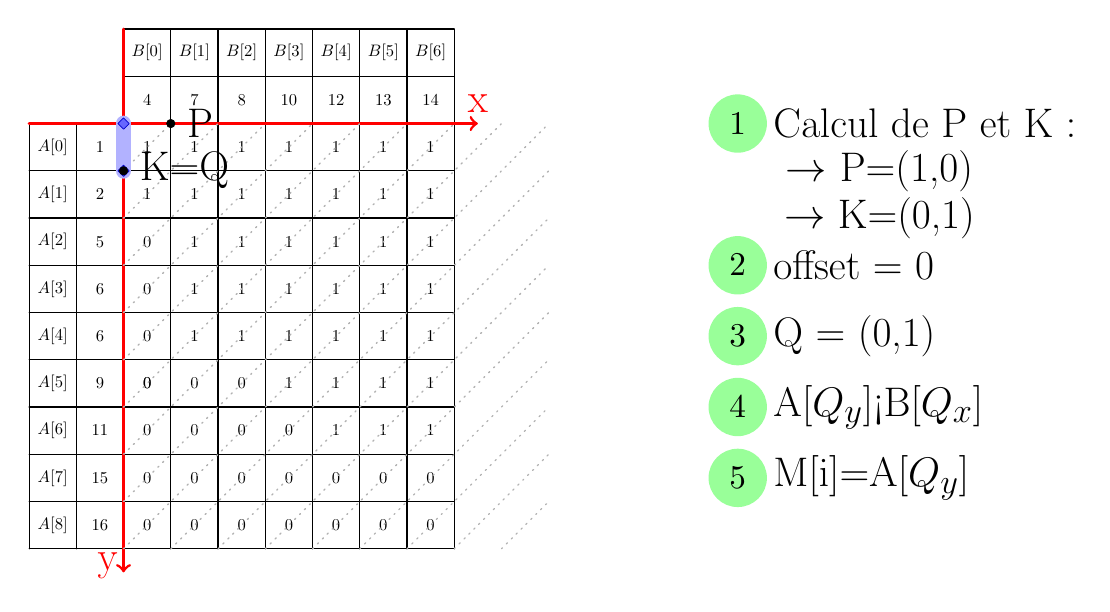
\begin{tikzpicture}[line cap=round,scale=0.6, every node/.style={transform shape}]
    \baseGraph
    \maze (-3,6) node {\BlueRoute}--(-3,5)node {\BlueRoute}; %ajouter ce qu'on a déjà fait 
    \draw (10,6) node[shape = circle,label=right:\Huge{Calcul de P et K :},fill=green!40,scale=2] {1}; 
    \draw (13,5) node {\Huge{$\rightarrow$ P=(1,0)}}; 
    \draw (-2,6) node[label=right:\Huge{P}] {\BlackCirc};

    \draw (13,4) node {\Huge{$\rightarrow$ K=(0,1)}};
    \draw (-3,5) node[label=right:\Huge{K=Q}] {\BlackCirc};
    \draw (10,3) node[shape = circle,label=right:\Huge{offset = 0},fill=green!40,scale=2] {2};
    \draw (10,1.5) node[shape = circle,label=right:\Huge{Q = (0,1)},fill=green!40,scale=2] {3};\pause
    \draw (10,0) node[shape = circle,label=right:\Huge{A[$Q_{y}$]<B[$Q_{x}$]},fill=green!40,scale=2] {4};\pause 
    \draw (10,-1.5) node[shape = circle,label=right:\Huge{M[i]=A[$Q_{y}$]},fill=green!40,scale=2] {5}; 
    %\draw (-3,6) node {\BlueRoute}; \pause
\end{tikzpicture}
\end{frame}


\begin{frame}{Path merged : thread 1, path}
    \setbeamercovered{invisible}
\RaggedRight
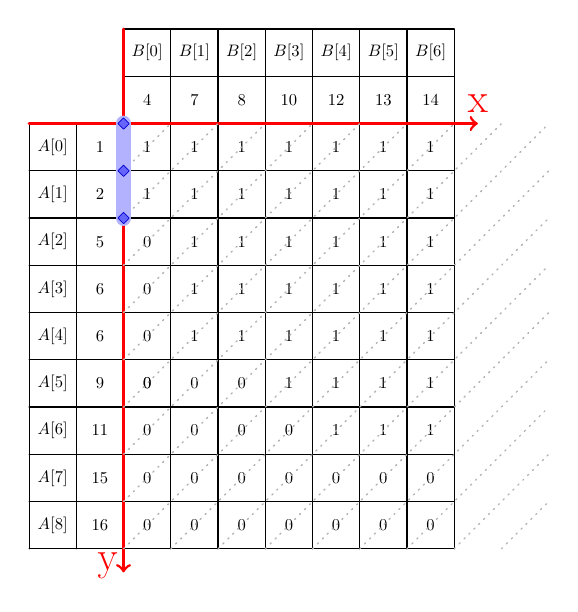
\begin{tikzpicture}[line cap=round,scale=0.6, every node/.style={transform shape}]
    \baseGraph
    \draw (-3,6) node {\BlueRoute}; 
    \maze (-3,6) node {\BlueRoute}--(-3,5)node {\BlueRoute};\pause
    \maze (-3,5) node {\BlueRoute}--(-3,4)node {\BlueRoute};
\end{tikzpicture}
\end{frame}
\begin{frame}{Path merged : thread 2}
    \setbeamercovered{invisible}
\RaggedRight
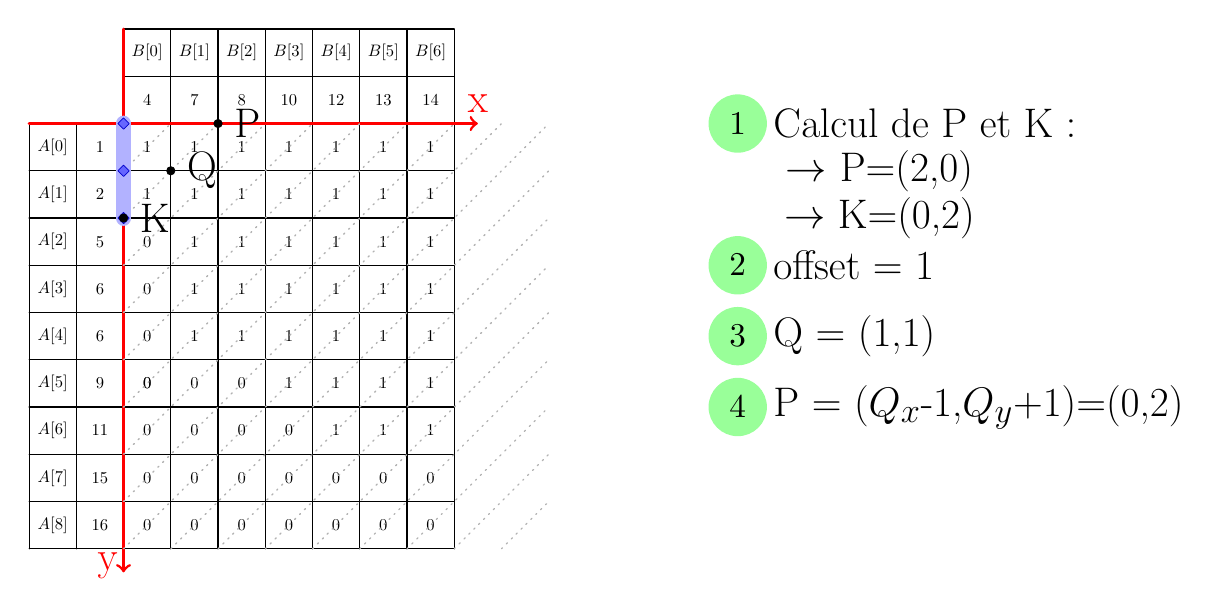
\begin{tikzpicture}[line cap=round,scale=0.6, every node/.style={transform shape}]
    \baseGraph
    \maze (-3,6) node {\BlueRoute}--(-3,5)node {\BlueRoute};
    \maze (-3,5) node {\BlueRoute}--(-3,4)node {\BlueRoute}; %ajouter ce qu'on a déjà fait 
    \draw (10,6) node[shape = circle,label=right:\Huge{Calcul de P et K :},fill=green!40,scale=2] {1};\pause 
    \draw (13,5) node {\Huge{$\rightarrow$ P=(2,0)}}; 
    \draw (-1,6) node[label=right:\Huge{P}] {\BlackCirc};\pause
    \draw (13,4) node {\Huge{$\rightarrow$ K=(0,2)}};
    \draw (-3,4) node[label=right:\Huge{K}] {\BlackCirc};\pause
    \draw (10,3) node[shape = circle,label=right:\Huge{offset = 1},fill=green!40,scale=2] {2};\pause
    \draw (10,1.5) node[shape = circle,label=right:\Huge{Q = (1,1)},fill=green!40,scale=2] {3};
    \draw (-2,5) node[label=right:\Huge{Q}] {\BlackCirc};\pause
    \draw (10,0) node[shape = circle,label=right:\Huge{P = ($Q_{x}$-1,$Q_{y}$+1)=(0,2)},fill=green!40,scale=2] {4};\pause 
    %\draw (10,-1.5) node[shape = circle,label=right:\Huge{M[i]=A[$Q_{y}$]},fill=green!40,scale=2] {5}; 
    %\draw (-3,6) node {\BlueRoute}; \pause
\end{tikzpicture}
\end{frame}



\begin{frame}{Path merged : thread 2}
    \setbeamercovered{invisible}
\RaggedRight
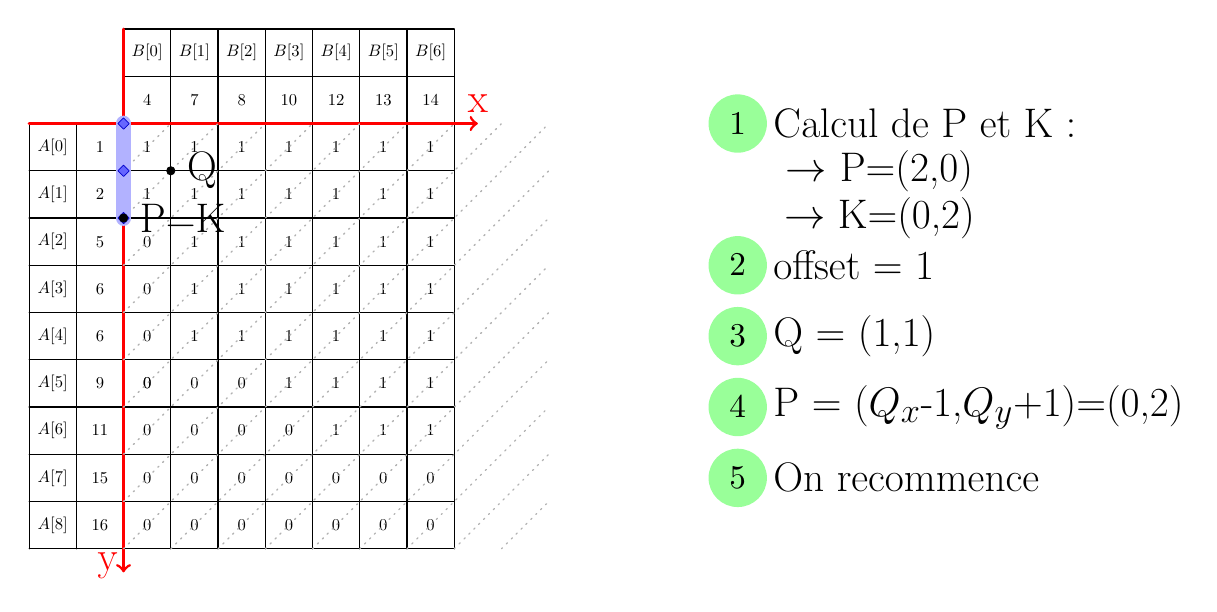
\begin{tikzpicture}[line cap=round,scale=0.6, every node/.style={transform shape}]
    \baseGraph
    \maze (-3,6) node {\BlueRoute}--(-3,5)node {\BlueRoute};
    \maze (-3,5) node {\BlueRoute}--(-3,4)node {\BlueRoute}; %ajouter ce qu'on a déjà fait 
    \draw (10,6) node[shape = circle,label=right:\Huge{Calcul de P et K :},fill=green!40,scale=2] {1}; 
    \draw (13,5) node {\Huge{$\rightarrow$ P=(2,0)}}; 
    \draw (-3,4) node[label=right:\Huge{P=K}] {\BlackCirc};
    \draw (13,4) node {\Huge{$\rightarrow$ K=(0,2)}};
    \draw (10,3) node[shape = circle,label=right:\Huge{offset = 1},fill=green!40,scale=2] {2};
    \draw (10,1.5) node[shape = circle,label=right:\Huge{Q = (1,1)},fill=green!40,scale=2] {3};
    \draw (-2,5) node[label=right:\Huge{Q}] {\BlackCirc};
    \draw (10,0) node[shape = circle,label=right:\Huge{P = ($Q_{x}$-1,$Q_{y}$+1)=(0,2)},fill=green!40,scale=2] {4};\pause 
    \draw (10,-1.5) node[shape = circle,label=right:\Huge{On recommence},fill=green!40,scale=2] {5}; 
    %\draw (-3,6) node {\BlueRoute}; \pause
\end{tikzpicture}
\end{frame}
\begin{frame}{Path merged : thread 2}
    \setbeamercovered{invisible}
\RaggedRight
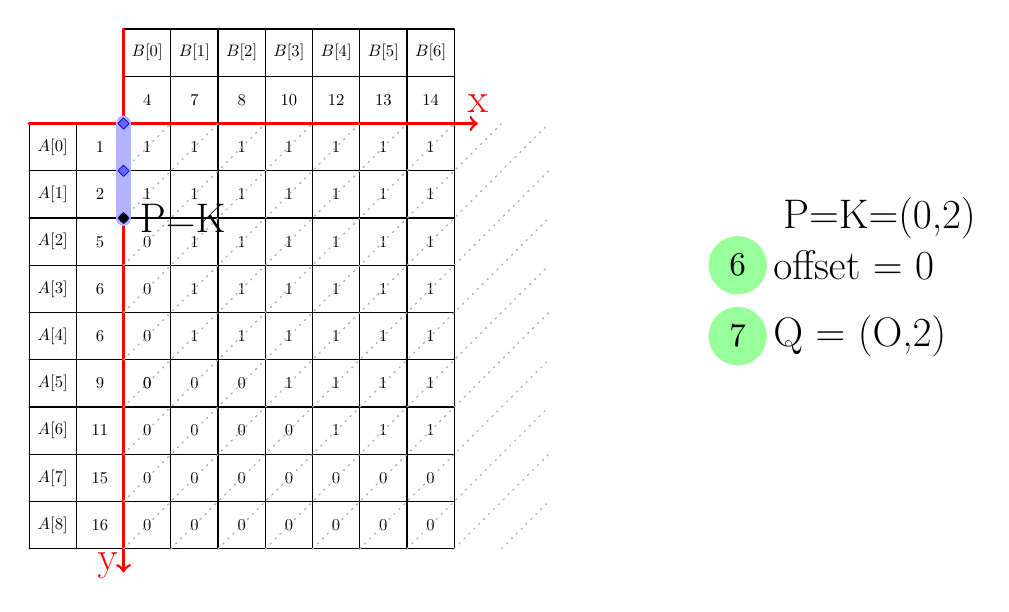
\begin{tikzpicture}[line cap=round,scale=0.6, every node/.style={transform shape}]
    \baseGraph
    \maze (-3,6) node {\BlueRoute}--(-3,5)node {\BlueRoute};
    \maze (-3,5) node {\BlueRoute}--(-3,4)node {\BlueRoute}; %ajouter ce qu'on a déjà fait 
 
    \draw (-3,4) node[label=right:\Huge{P=K}] {\BlackCirc};
    \draw (13,4) node {\Huge{P=K=(0,2)}};
    \draw (10,3) node[shape = circle,label=right:\Huge{offset = 0},fill=green!40,scale=2] {6};\pause
    \draw (10,1.5) node[shape = circle,label=right:\Huge{Q = (O,2)},fill=green!40,scale=2] {7};
\end{tikzpicture}
\end{frame}


\begin{frame}{Path merged : thread 2}
    \setbeamercovered{invisible}
\RaggedRight
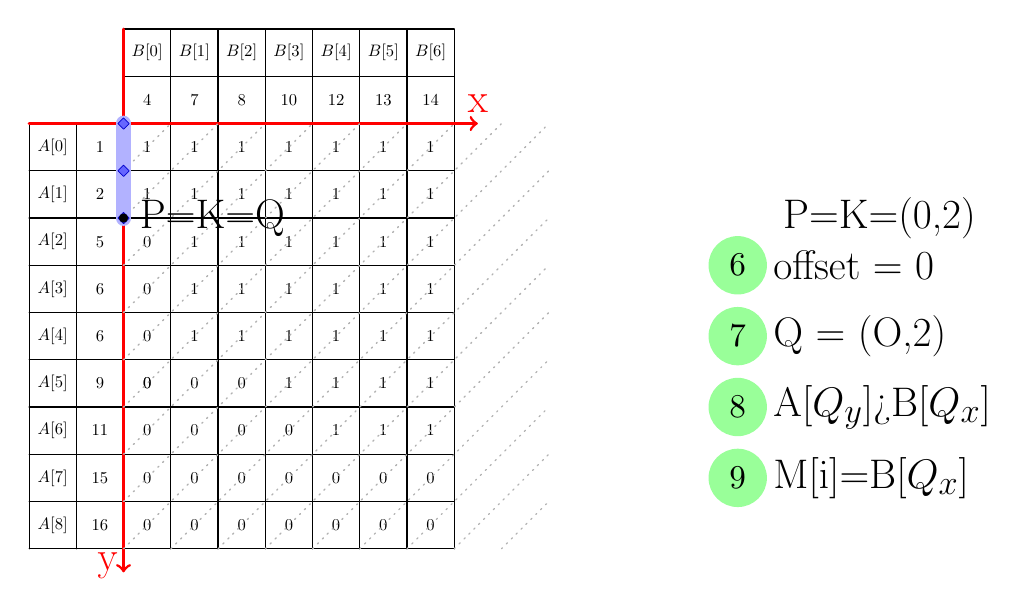
\begin{tikzpicture}[line cap=round,scale=0.6, every node/.style={transform shape}]
    \baseGraph
    \maze (-3,6) node {\BlueRoute}--(-3,5)node {\BlueRoute};
    \maze (-3,5) node {\BlueRoute}--(-3,4)node {\BlueRoute}; %ajouter ce qu'on a déjà fait 
 
    \draw (-3,4) node[label=right:\Huge{P=K=Q}] {\BlackCirc};
    \draw (13,4) node {\Huge{P=K=(0,2)}};
    \draw (10,3) node[shape = circle,label=right:\Huge{offset = 0},fill=green!40,scale=2] {6};
    \draw (10,1.5) node[shape = circle,label=right:\Huge{Q = (O,2)},fill=green!40,scale=2] {7};
    \draw (10,0) node[shape = circle,label=right:\Huge{A[$Q_{y}$]>B[$Q_{x}$]},fill=green!40,scale=2] {8};\pause 
    \draw (10,-1.5) node[shape = circle,label=right:\Huge{M[i]=B[$Q_{x}$]},fill=green!40,scale=2] {9}; 
\end{tikzpicture}
\end{frame}



\begin{frame}{Path merged : thread 2, path}
    \setbeamercovered{invisible}
\RaggedRight
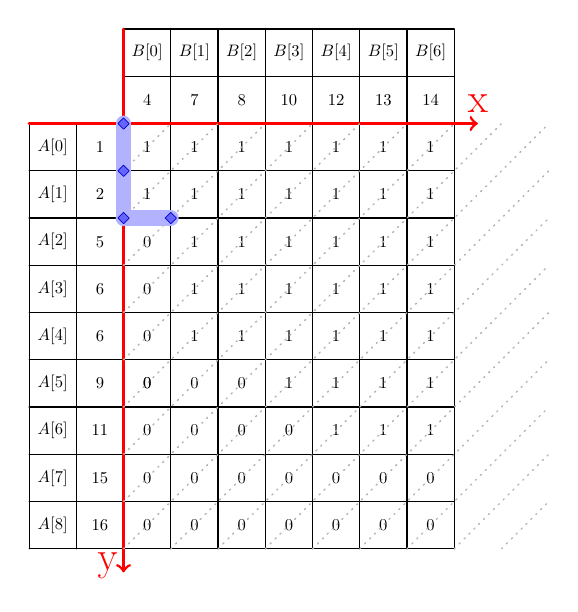
\begin{tikzpicture}[line cap=round,scale=0.6, every node/.style={transform shape}]
    \baseGraph
    \draw (-3,6) node {\BlueRoute}; 
    \maze (-3,6) node {\BlueRoute}--(-3,5)node {\BlueRoute};
    \maze (-3,5) node {\BlueRoute}--(-3,4)node {\BlueRoute};\pause
    \maze (-3,4) node {\BlueRoute}--(-2,4)node {\BlueRoute};
\end{tikzpicture}
\end{frame}
\begin{frame}{Skipping to thread 9}
    \setbeamercovered{invisible}
\RaggedRight
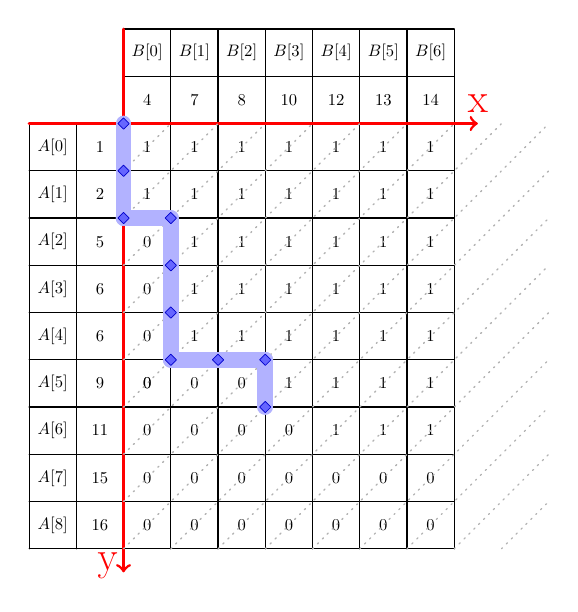
\begin{tikzpicture}[line cap=round,scale=0.6, every node/.style={transform shape}]
    \baseGraph
    \draw (-3,6) node {\BlueRoute}; 
    \maze (-3,6) node {\BlueRoute}--(-3,5)node {\BlueRoute};
    \maze (-3,5) node {\BlueRoute}--(-3,4)node {\BlueRoute};
    \maze (-3,4) node {\BlueRoute}--(-2,4)node {\BlueRoute};
    \maze (-2,4) node {\BlueRoute}--(-2,3)node {\BlueRoute};\pause
    \maze (-2,3) node {\BlueRoute}--(-2,2)node {\BlueRoute};\pause
    \maze (-2,2) node {\BlueRoute}--(-2,1)node {\BlueRoute};\pause
    \maze (-2,1) node {\BlueRoute}--(-1,1) node {\BlueRoute};
    \maze (-1,1) node {\BlueRoute}--(0,1) node {\BlueRoute};
    \maze (0,1)  node {\BlueRoute}--(0,0) node {\BlueRoute};\pause
\end{tikzpicture}
\end{frame}

\begin{frame}{Path merged : thread 9}
    \setbeamercovered{invisible}
\RaggedRight
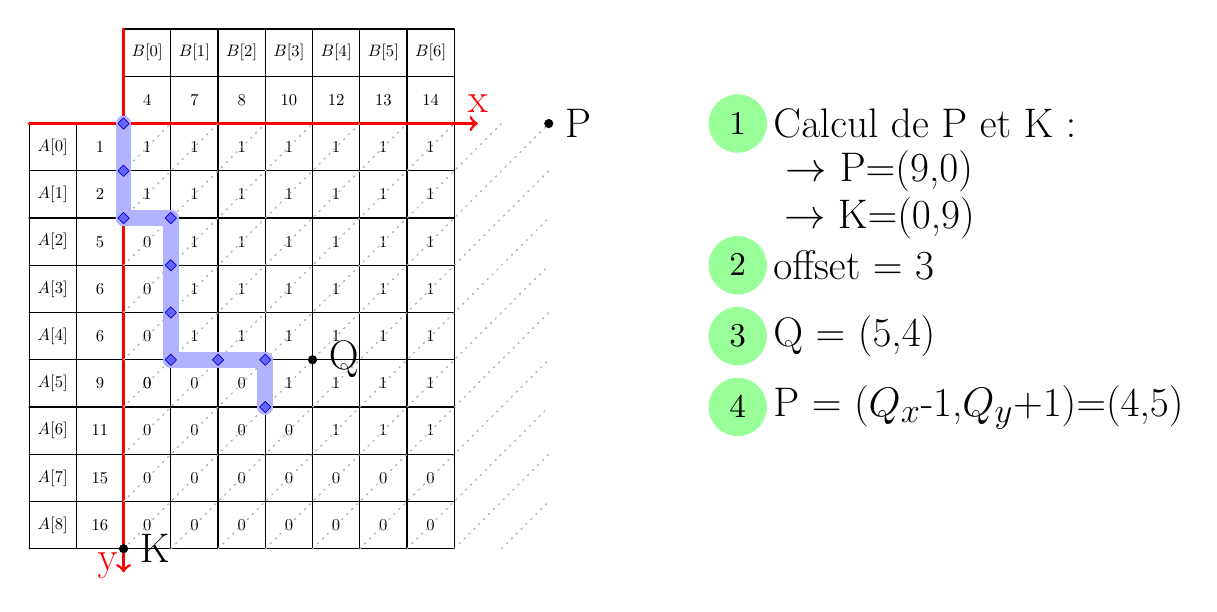
\begin{tikzpicture}[line cap=round,scale=0.6, every node/.style={transform shape}]
    \baseGraph
    \draw (-3,6) node {\BlueRoute}; 
    \maze (-3,6) node {\BlueRoute}--(-3,5)node {\BlueRoute};
    \maze (-3,5) node {\BlueRoute}--(-3,4)node {\BlueRoute};
    \maze (-3,4) node {\BlueRoute}--(-2,4)node {\BlueRoute};
    \maze (-2,4) node {\BlueRoute}--(-2,3)node {\BlueRoute};
    \maze (-2,3) node {\BlueRoute}--(-2,2)node {\BlueRoute};
    \maze (-2,2) node {\BlueRoute}--(-2,1)node {\BlueRoute};
    \maze (-2,1) node {\BlueRoute}--(-1,1) node {\BlueRoute};
    \maze (-1,1) node {\BlueRoute}--(0,1) node {\BlueRoute};
    \maze (0,1)  node {\BlueRoute}--(0,0) node {\BlueRoute}; %ajouter ce qu'on a déjà fait 
    \draw (10,6) node[shape = circle,label=right:\Huge{Calcul de P et K :},fill=green!40,scale=2] {1};\pause 
    \draw (13,5) node {\Huge{$\rightarrow$ P=(9,0)}}; 
    \draw (6,6) node[label=right:\Huge{P}] {\BlackCirc};\pause
    \draw (13,4) node {\Huge{$\rightarrow$ K=(0,9)}};
    \draw (-3,-3) node[label=right:\Huge{K}] {\BlackCirc};\pause
    \draw (10,3) node[shape = circle,label=right:\Huge{offset = 3},fill=green!40,scale=2] {2};\pause
    \draw (10,1.5) node[shape = circle,label=right:\Huge{Q = (5,4)},fill=green!40,scale=2] {3};
    \draw (1,1) node[label=right:\Huge{Q}] {\BlackCirc};\pause
    \draw (10,0) node[shape = circle,label=right:\Huge{P = ($Q_{x}$-1,$Q_{y}$+1)=(4,5)},fill=green!40,scale=2] {4};\pause 
    %\draw (10,-1.5) node[shape = circle,label=right:\Huge{M[i]=A[$Q_{y}$]},fill=green!40,scale=2] {5}; 
    %\draw (-3,6) node {\BlueRoute}; \pause
\end{tikzpicture}
\end{frame}


\begin{frame}{Path merged : thread 9}
    \setbeamercovered{invisible}
\RaggedRight
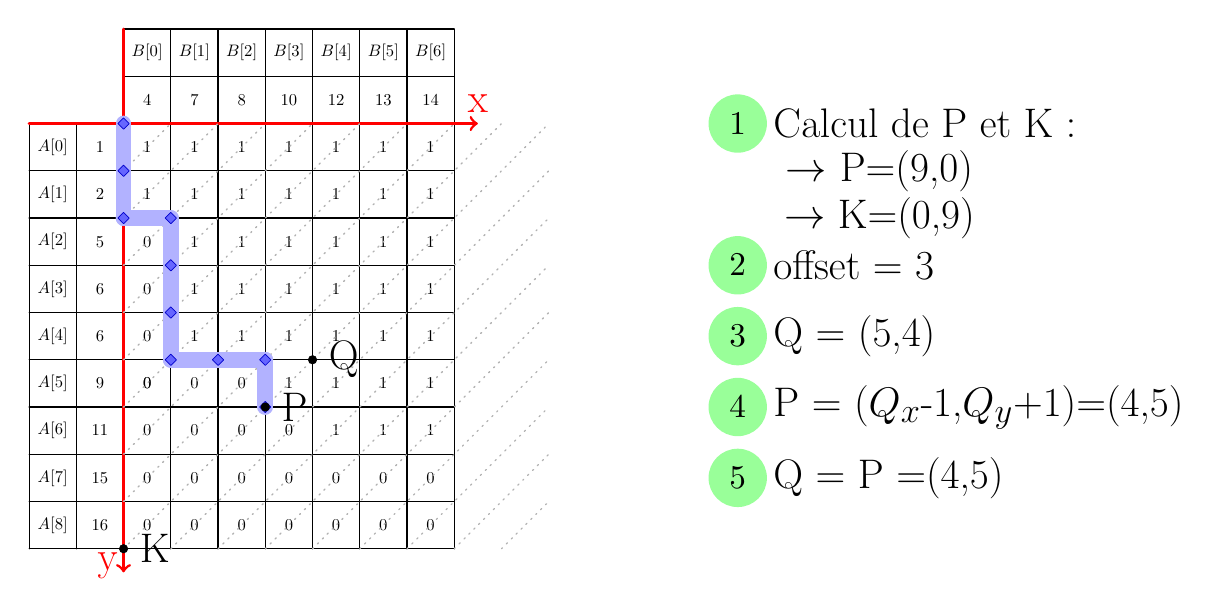
\begin{tikzpicture}[line cap=round,scale=0.6, every node/.style={transform shape}]
    \baseGraph
    \draw (-3,6) node {\BlueRoute}; 
    \maze (-3,6) node {\BlueRoute}--(-3,5)node {\BlueRoute};
    \maze (-3,5) node {\BlueRoute}--(-3,4)node {\BlueRoute};
    \maze (-3,4) node {\BlueRoute}--(-2,4)node {\BlueRoute};
    \maze (-2,4) node {\BlueRoute}--(-2,3)node {\BlueRoute};
    \maze (-2,3) node {\BlueRoute}--(-2,2)node {\BlueRoute};
    \maze (-2,2) node {\BlueRoute}--(-2,1)node {\BlueRoute};
    \maze (-2,1) node {\BlueRoute}--(-1,1) node {\BlueRoute};
    \maze (-1,1) node {\BlueRoute}--(0,1) node {\BlueRoute};
    \maze (0,1)  node {\BlueRoute}--(0,0) node {\BlueRoute}; %ajouter ce qu'on a déjà fait 
    \draw (10,6) node[shape = circle,label=right:\Huge{Calcul de P et K :},fill=green!40,scale=2] {1}; 
    \draw (13,5) node {\Huge{$\rightarrow$ P=(9,0)}}; 
    \draw (0,0) node[label=right:\Huge{P}] {\BlackCirc};
    \draw (13,4) node {\Huge{$\rightarrow$ K=(0,9)}};
    \draw (-3,-3) node[label=right:\Huge{K}] {\BlackCirc};
    \draw (10,3) node[shape = circle,label=right:\Huge{offset = 3},fill=green!40,scale=2] {2};
    \draw (10,1.5) node[shape = circle,label=right:\Huge{Q = (5,4)},fill=green!40,scale=2] {3};
    \draw (1,1) node[label=right:\Huge{Q}] {\BlackCirc};
    \draw (10,0) node[shape = circle,label=right:\Huge{P = ($Q_{x}$-1,$Q_{y}$+1)=(4,5)},fill=green!40,scale=2] {4}; 
    \draw (10,-1.5) node[shape = circle,label=right:\Huge{Q = P =(4,5)},fill=green!40,scale=2] {5}; 
    %\draw (10,-1.5) node[shape = circle,label=right:\Huge{M[i]=A[$Q_{y}$]},fill=green!40,scale=2] {5}; 
    %\draw (-3,6) node {\BlueRoute}; \pause
\end{tikzpicture}
\end{frame}

\begin{frame}{Path merged : thread 9}
    \setbeamercovered{invisible}
\RaggedRight
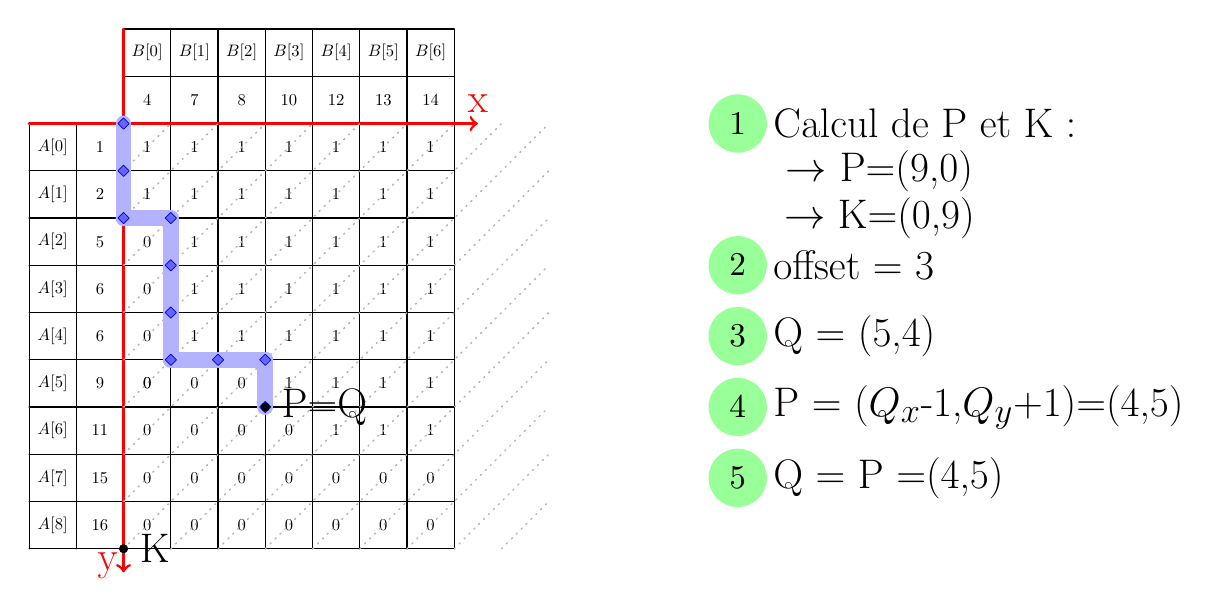
\begin{tikzpicture}[line cap=round,scale=0.6, every node/.style={transform shape}]
    \baseGraph
    \draw (-3,6) node {\BlueRoute}; 
    \maze (-3,6) node {\BlueRoute}--(-3,5)node {\BlueRoute};
    \maze (-3,5) node {\BlueRoute}--(-3,4)node {\BlueRoute};
    \maze (-3,4) node {\BlueRoute}--(-2,4)node {\BlueRoute};
    \maze (-2,4) node {\BlueRoute}--(-2,3)node {\BlueRoute};
    \maze (-2,3) node {\BlueRoute}--(-2,2)node {\BlueRoute};
    \maze (-2,2) node {\BlueRoute}--(-2,1)node {\BlueRoute};
    \maze (-2,1) node {\BlueRoute}--(-1,1) node {\BlueRoute};
    \maze (-1,1) node {\BlueRoute}--(0,1) node {\BlueRoute};
    \maze (0,1)  node {\BlueRoute}--(0,0) node {\BlueRoute}; %ajouter ce qu'on a déjà fait 
    \draw (10,6) node[shape = circle,label=right:\Huge{Calcul de P et K :},fill=green!40,scale=2] {1}; 
    \draw (13,5) node {\Huge{$\rightarrow$ P=(9,0)}}; 
    \draw (13,4) node {\Huge{$\rightarrow$ K=(0,9)}};
    \draw (-3,-3) node[label=right:\Huge{K}] {\BlackCirc};
    \draw (10,3) node[shape = circle,label=right:\Huge{offset = 3},fill=green!40,scale=2] {2};
    \draw (10,1.5) node[shape = circle,label=right:\Huge{Q = (5,4)},fill=green!40,scale=2] {3};
    \draw (0,0) node[label=right:\Huge{P=Q}] {\BlackCirc};
    \draw (10,0) node[shape = circle,label=right:\Huge{P = ($Q_{x}$-1,$Q_{y}$+1)=(4,5)},fill=green!40,scale=2] {4}; 
    \draw (10,-1.5) node[shape = circle,label=right:\Huge{Q = P =(4,5)},fill=green!40,scale=2] {5}; 
    %\draw (10,-1.5) node[shape = circle,label=right:\Huge{M[i]=A[$Q_{y}$]},fill=green!40,scale=2] {5}; 
    %\draw (-3,6) node {\BlueRoute}; \pause
\end{tikzpicture}
\end{frame}

\begin{frame}{Path merged : thread 9}
    \setbeamercovered{invisible}
\RaggedRight
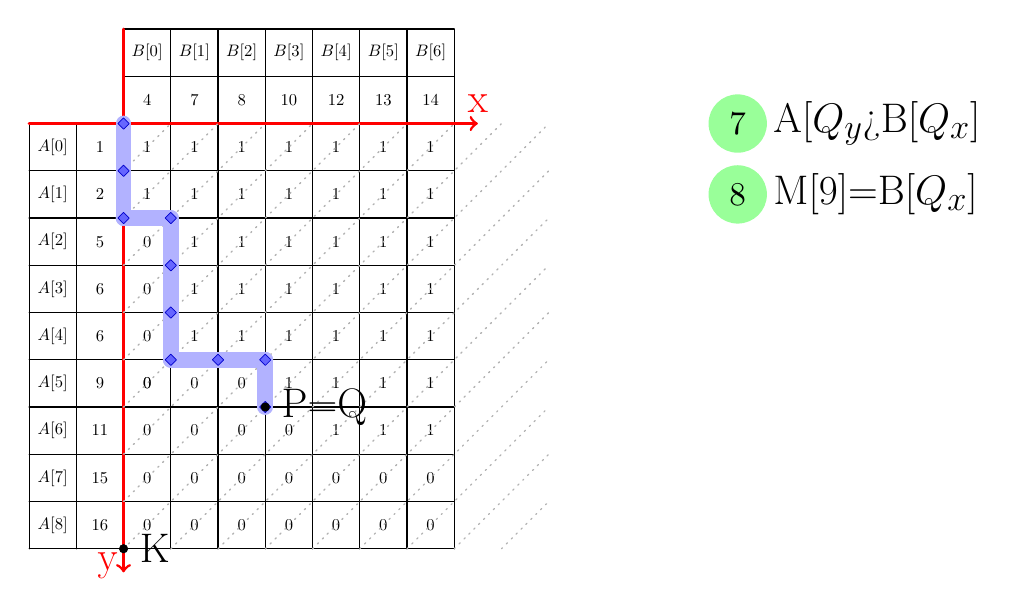
\begin{tikzpicture}[line cap=round,scale=0.6, every node/.style={transform shape}]
    \baseGraph
    \draw (-3,6) node {\BlueRoute}; 
    \maze (-3,6) node {\BlueRoute}--(-3,5)node {\BlueRoute};
    \maze (-3,5) node {\BlueRoute}--(-3,4)node {\BlueRoute};
    \maze (-3,4) node {\BlueRoute}--(-2,4)node {\BlueRoute};
    \maze (-2,4) node {\BlueRoute}--(-2,3)node {\BlueRoute};
    \maze (-2,3) node {\BlueRoute}--(-2,2)node {\BlueRoute};
    \maze (-2,2) node {\BlueRoute}--(-2,1)node {\BlueRoute};
    \maze (-2,1) node {\BlueRoute}--(-1,1) node {\BlueRoute};
    \maze (-1,1) node {\BlueRoute}--(0,1) node {\BlueRoute};
    \maze (0,1)  node {\BlueRoute}--(0,0) node {\BlueRoute}; %ajouter ce qu'on a déjà fait 
    \draw (-3,-3) node[label=right:\Huge{K}] {\BlackCirc};
    \draw (0,0) node[label=right:\Huge{P=Q}] {\BlackCirc};
    \draw (10,6) node[shape = circle,label=right:\Huge{A[$Q_{y}$>B[$Q_{x}$]},fill=green!40,scale=2] {7}; \pause
    \draw (10,4.5) node[shape = circle,label=right:\Huge{M[9]=B[$Q_{x}$]},fill=green!40,scale=2] {8};\pause
\end{tikzpicture}
\end{frame}


\begin{frame}{Path merged : thread 9, path}
    \setbeamercovered{invisible}
\RaggedRight
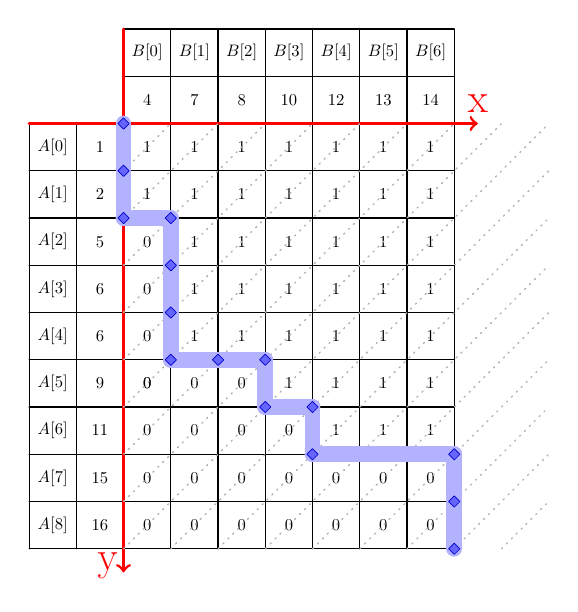
\begin{tikzpicture}[line cap=round,scale=0.6, every node/.style={transform shape}]
    \baseGraph
    \draw (-3,6) node {\BlueRoute}; 
    \maze (-3,6) node {\BlueRoute}--(-3,5)node {\BlueRoute};
    \maze (-3,5) node {\BlueRoute}--(-3,4)node {\BlueRoute};
    \maze (-3,4) node {\BlueRoute}--(-2,4)node {\BlueRoute};
    \maze (-2,4) node {\BlueRoute}--(-2,3)node {\BlueRoute};
    \maze (-2,3) node {\BlueRoute}--(-2,2)node {\BlueRoute};
    \maze (-2,2) node {\BlueRoute}--(-2,1)node {\BlueRoute};
    \maze (-2,1) node {\BlueRoute}--(-1,1) node {\BlueRoute};
    \maze (-1,1) node {\BlueRoute}--(0,1) node {\BlueRoute};
    \maze (0,1)  node {\BlueRoute}--(0,0) node {\BlueRoute};
    \maze (0,0)  node {\BlueRoute}--(1,0) node {\BlueRoute};\pause
    \maze (1,0)  node {\BlueRoute}--(1,-1)node {\BlueRoute};\pause
    \maze (1,-1) node {\BlueRoute}--(4,-1)node {\BlueRoute};\pause
    \maze (4,-1) node {\BlueRoute}--(4,-2)node {\BlueRoute};\pause
    \maze (4,-2) node {\BlueRoute}--(4,-3)node {\BlueRoute};\pause
    
\end{tikzpicture}
\end{frame}


\end{document}